\section{Quantization}
\label{sec:quantization}

After post-training the model in BF16, we applied Post-Training Quantization (PTQ) using \mbox{ModelOpt}\footnote{\url{https://github.com/NVIDIA/Model-Optimizer}} and Megatron-LM to quantize the model to FP8.

\subsection{Post-Training Quantization Calibration Dataset}
For PTQ calibration, we used a small subset containing 1K samples from post-training reasoning SFT dataset. Using calibration data based on the post-training SFT data yielded slightly better accuracy recovery compared to the \texttt{cnn\_dailymail} dataset.

We also ablated with PTQ using calibration data curated from on-policy generations from the BF16 model, but did not observe any benefit in accuracy recovery compared to the SFT-based calibration dataset. 

\subsection{Selective Post-Training Quantization}
To preserve accuracy while improving efficiency, we used a selective quantization strategy.
%
We performed quantization sensitivity analysis and explored a set of quantization configurations for mixed-precision models. This study showed that self-attention layers (6 out of 52 layers for \ourmodel) are the most sensitive components, hence we keep them in BF16. Also, the Mamba layers that feed into the self-attention layers were found to be sensitive and are kept in BF16. Overall, keeping the 6 self-attention layers and the 6 Mamba layers in BF16 provided a sweet-spot configuration for accuracy recovery and efficiency trade-off.

The model weights, activations, and KV cache are quantized to FP8. Conv1D within all the Mamba layers are kept in BF16. %The MoE router is not quantized, and kept in FP32 precision.

\subsection{Accuracy and Throughput} 
\label{subsec:quantaccuracy}
Table~\ref{tab:nano_v3_quant_accuracy} compares accuracy numbers of \ourmodel FP8 with BF16 on multiple benchmarks. Overall, the FP8 model achieves approximately 99\% median accuracy recovery compared to the BF16 model.

To verify the effectiveness of our selective quantization strategy and to better understand the accuracy–efficiency trade-off, we evaluated several quantization configurations. We conducted an ablation study by applying PTQ to different model components.
%
Specifically, we examined three factors: attention layer quantization (BF16 or FP8), Mamba layer quantization (FP8 or a mix of BF16 and FP8), and KV cache quantization (BF16 or FP8).

\begin{figure}[h]
    \centering
    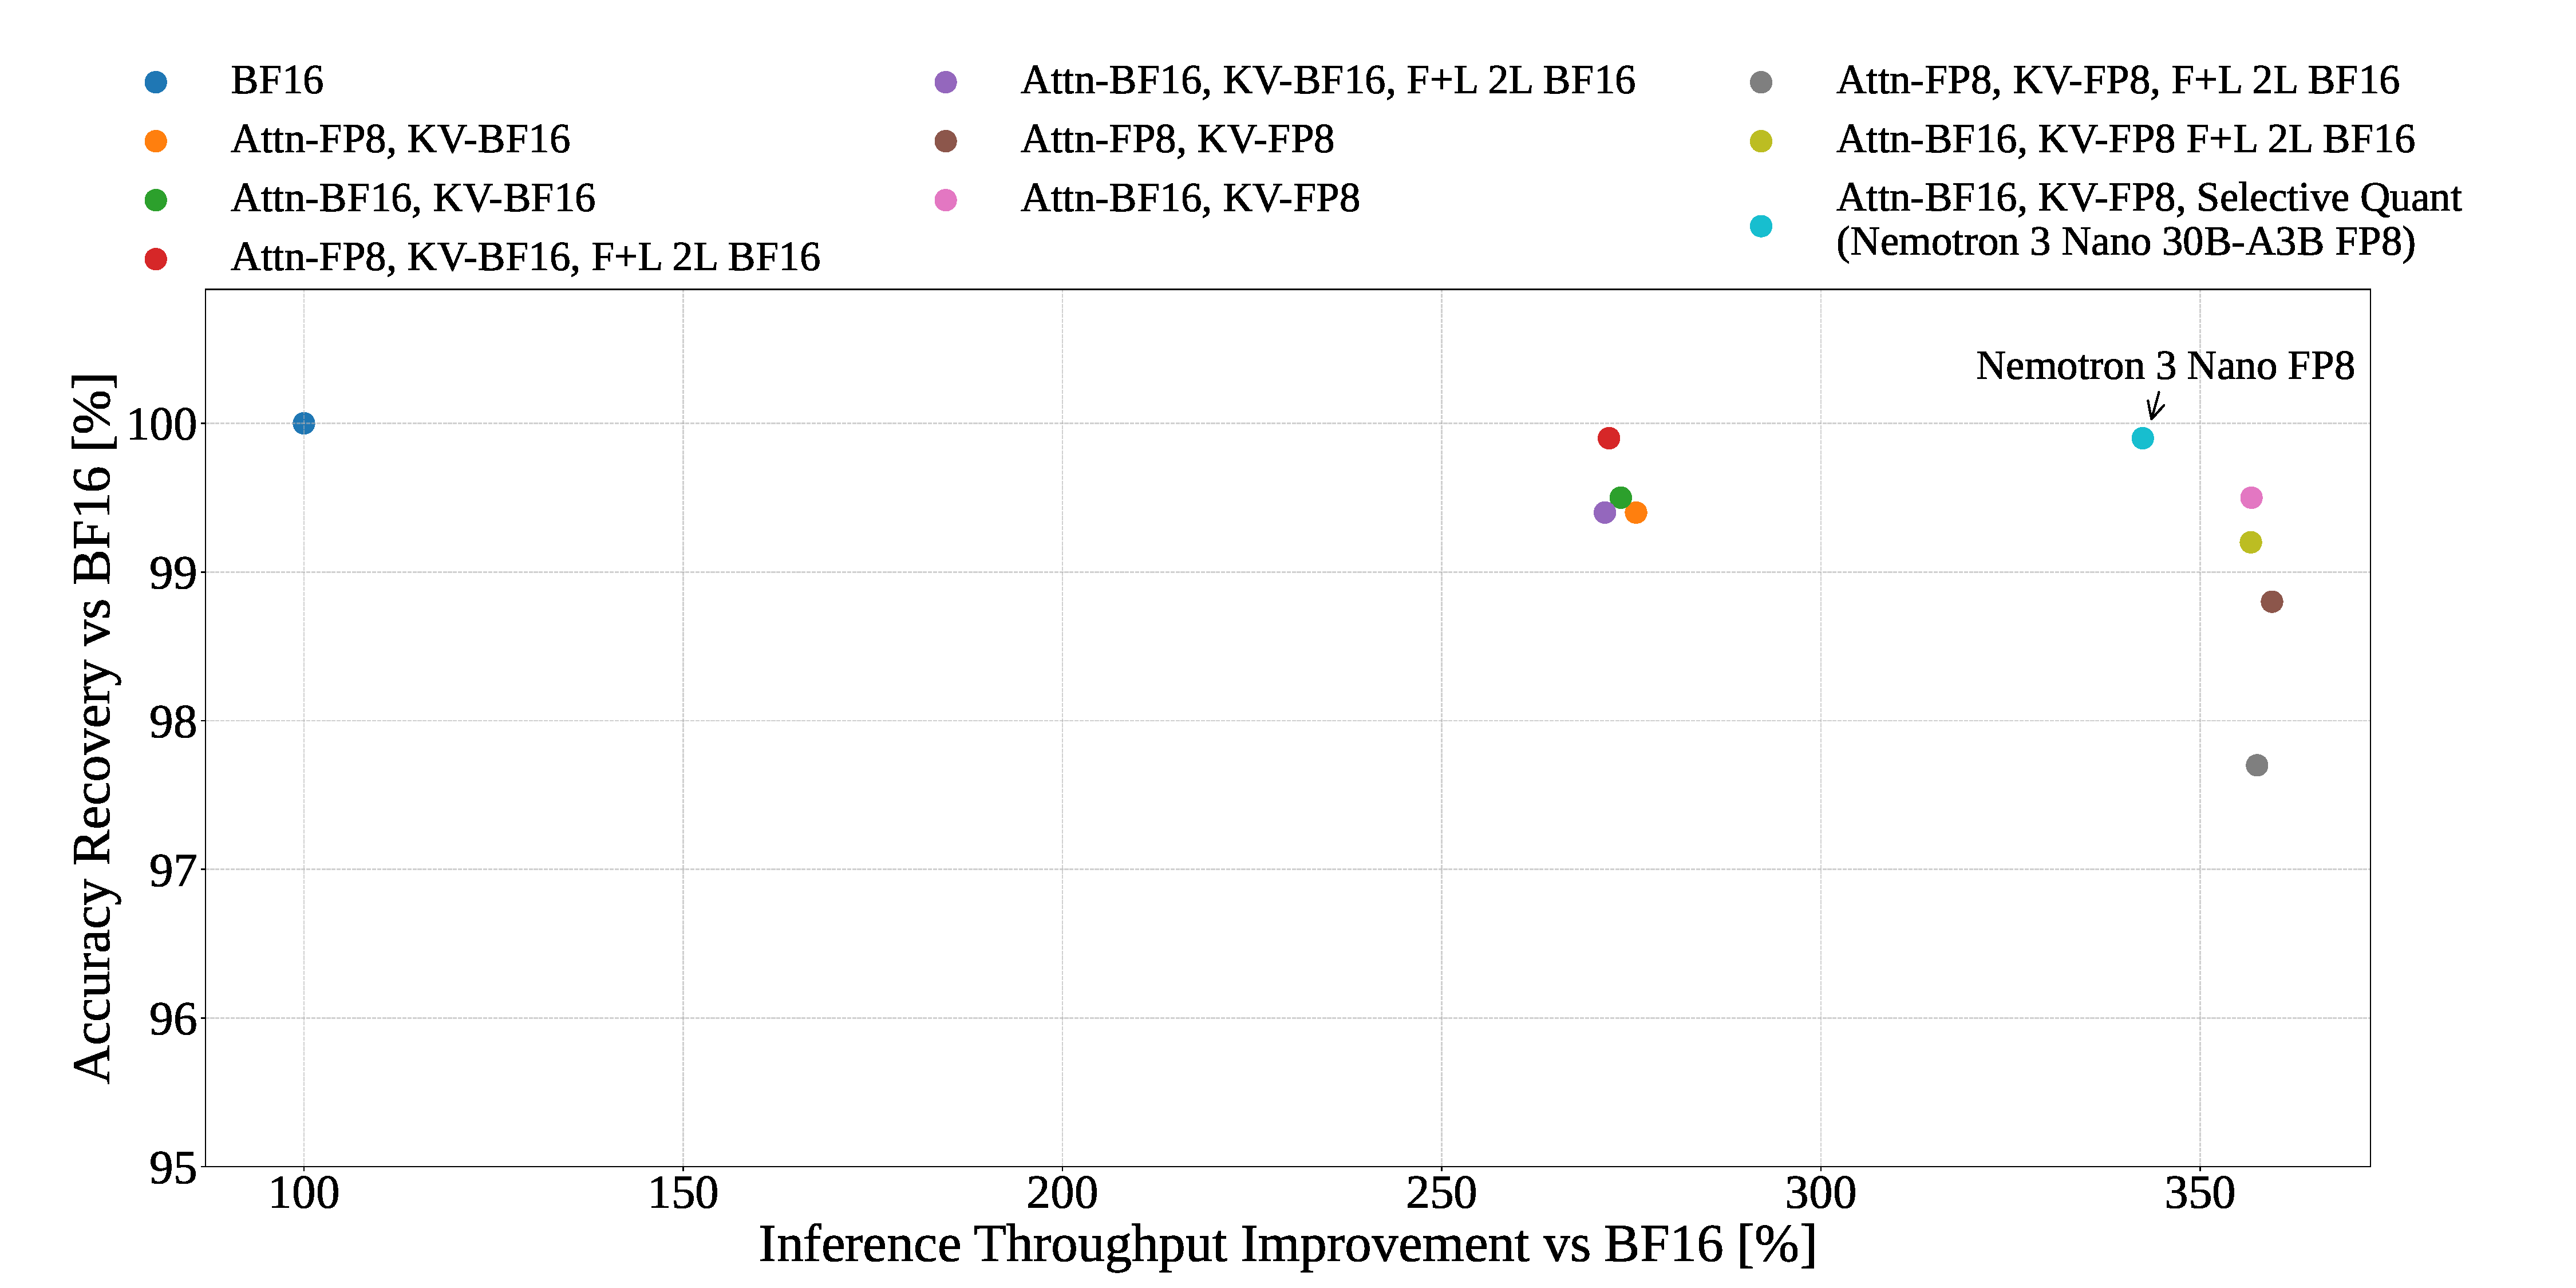
\includegraphics[width=\linewidth]{figures/fp8-acc-vs-throughput.pdf}
    \caption{Ablation study of different quantization configurations for accuracy–throughput trade-offs. Accuracy recovery and throughput improvements are computed relative to the \ourmodel{} BF16 checkpoint, with values normalized such that the BF16 baseline is 100\%. Accuracy recovery is defined as the median of the recovery rates across all benchmarks.
    %
    The benchmark was conducted on a single H100 with ISL/OSL=8K/16K. Given that more aggressively quantized models can accommodate larger batch sizes due to lower memory footprint, we used the maximum batch size for each quantization configuration for fair comparisons under the same hardware constraints.}
    \label{fig:fp8_acc_vs_throughput}
\end{figure}


As shown in Figure~\ref{fig:fp8_acc_vs_throughput}, KV cache with FP8 quantization significantly improves throughput by enabling larger batch sizes. While other quantization configurations suffer from accuracy degradation, our selective quantization can retain the accuracy numbers even with KV cache quantization. 
%
The results confirm that retaining the self-attention layers and their preceding Mamba layers in BF16, while quantizing the remaining layers and the KV cache in FP8, yields a strong accuracy–efficiency trade-off.

\begin{table*}[!htp]
\centering
\small
\setlength{\tabcolsep}{7pt}
\renewcommand{\arraystretch}{1.15}

\begin{tabular}{l|c c }
\toprule
\textbf{Benchmark} & \textbf{N-3-Nano BF16} & \textbf{N-3-Nano FP8} \\
\midrule
\rowcolor{black!5}
\multicolumn{3}{l}{\textbf{General Knowledge}} \\
MMLU-Pro &  78.30 & 78.10 \\

\midrule
\rowcolor{black!5}
\multicolumn{3}{l}{\textbf{Reasoning}} \\
AIME25 (no tools) & 89.06 & 87.71 \\
AIME25 (with tools) & 99.17 & 98.80 \\
GPQA (no tools) &  73.04 & 72.47 \\
GPQA (with tools) & 75.00 & 73.40  \\
% LiveCodeBench (v5 2024-07$\leftrightarrow$12) & 72.063 & - \\
LiveCodeBench (v6 2024-08$\leftrightarrow$2025-05) & 68.25 & 67.62 \\
SciCode (subtask) & 33.28 & 31.88 \\
HLE (no tools) & 10.57 & 10.33 \\
HLE (with tools) & 15.48 & 14.27  \\
%MiniF2F pass@1 & 50.0 & - \\
%MiniF2F pass@32 & 79.9 & - \\
\midrule
\rowcolor{black!5}
\multicolumn{3}{l}{\textbf{Agentic}} \\
%Terminal Bench (hard subset) & 8.5 & v \\
% Terminal Bench (nv-internal mix) &  &  &  \\
% SWE-Bench Verified & 38.760 & ?  \\
\textbf{TauBench V2} &  &   \\
\quad Airline & 48.00 & 44.79 \\
\quad Retail & 56.91 & 55.59 \\
\quad Telecom & 42.21 & 40.75 \\
\quad Average & 49.04 & 47.04 \\
BFCL v4 & 53.76 & 53.15 \\
\midrule
\rowcolor{black!5}
\multicolumn{3}{l}{\textbf{Chat \& Instruction Following}} \\
IFBench (prompt) & 71.51 & 72.19 \\
% IFBench (instruction) & 77.015 &  &  \\
%Scale AI Multi Challenge & 38.5  & - \\
% where does BF16 ArenaHard number come from?
%Arena-Hard-V2 (Hard Prompt) & 72.1 & - \\
%Arena-Hard-V2 (Creative Writing) & 63.2 &  - \\
%Arena-Hard-V2 (Average) & 67.7 & - \\

\midrule
\rowcolor{black!5}
\multicolumn{3}{l}{\textbf{Long Context}} \\
AA-LCR & 35.85 & 36.06 \\
%RULER-100 @ 256k & 92.9 & - \\
%RULER-100 @ 512K & 91.3 & -\\
%RULER-100 @ 1M & 86.3 & - \\

\midrule
\rowcolor{black!5}
\multicolumn{3}{l}{\textbf{Multilingual}} \\
MMLU-ProX (avg over langs) & 59.50 & 59.63 \\
% MMLU-ProX (avg over langs w/o Ja) &  &  &  \\
%WMT24++ (en$\rightarrow$xx) & 86.2 & - \\
% COMET?? & &  &  \\

\bottomrule
\end{tabular}

\caption{Accuracy numbers of \ourmodel{} before/after FP8 quantization.}

\label{tab:nano_v3_quant_accuracy}
\end{table*}



%% ===== UPDATED VERSION =======
